\chapter{Diagramme d'activités}

\section{Diagramme}

\begin{figure}
  \centering
  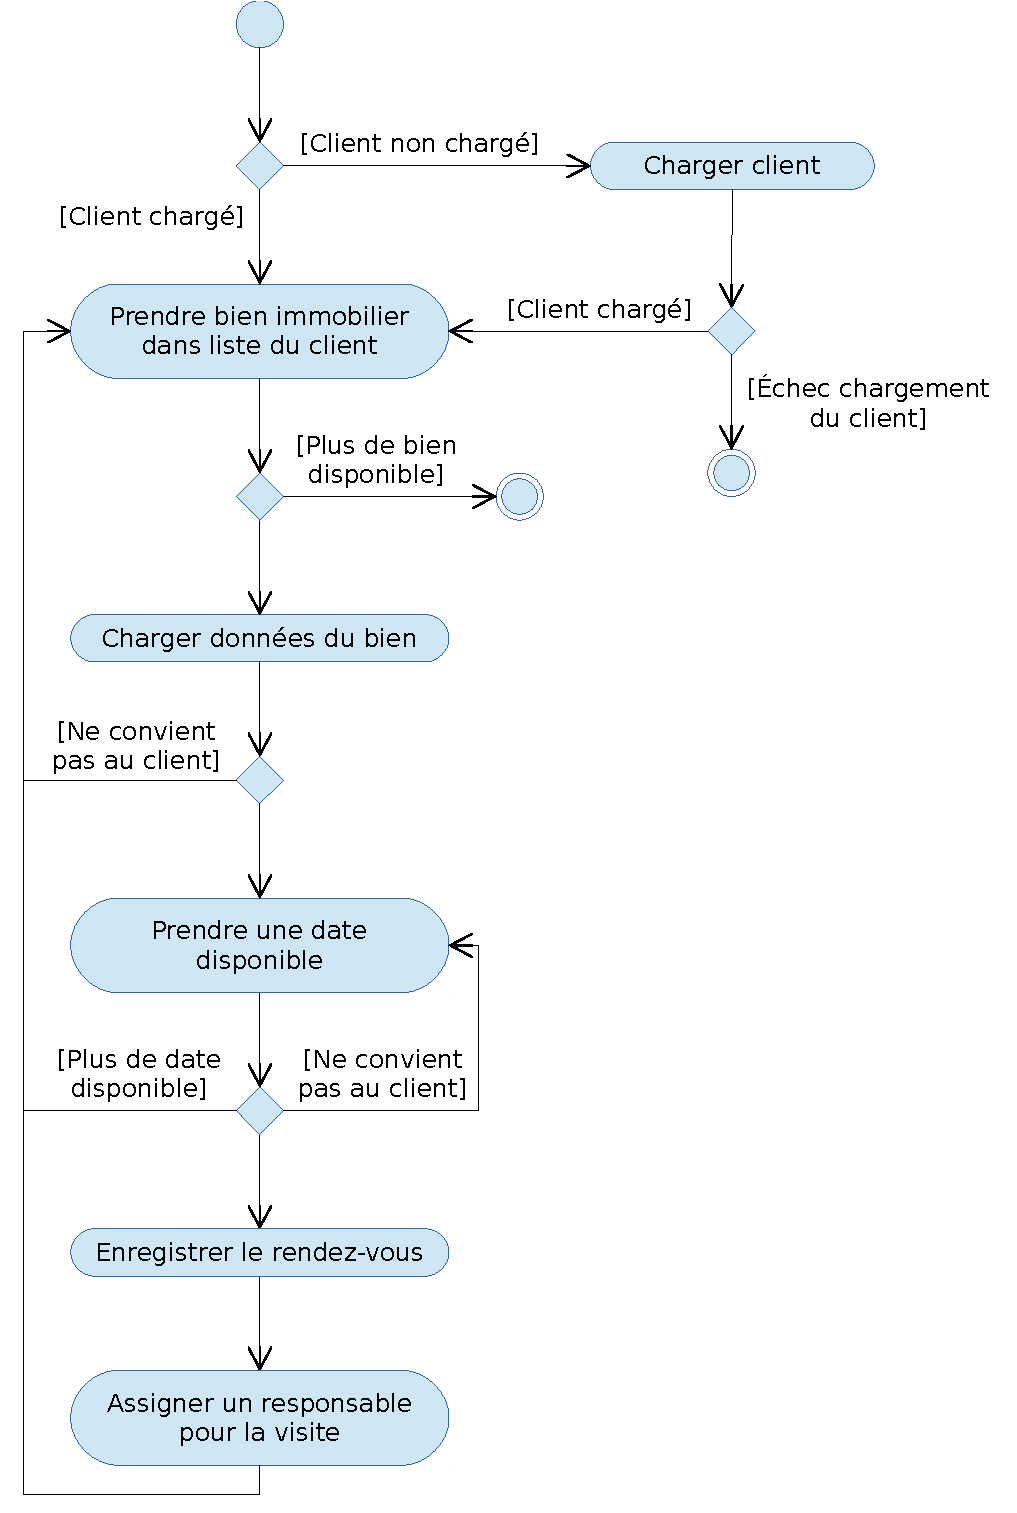
\includegraphics[scale=0.67]{IMG/ad}
  \caption{Diagramme d'activités}
  \label{img_ad}
\end{figure}

La figure \refpage{img_ad} illustre le diagramme d'activité du cas d'utilisation \og{}Visiter un bien\fg{}.

\section{Rapport}

Ce diagramme est basé sur le scénario du cas d'utilisation \og{}Visiter un bien\fg{}. Ce cas d'utilisation est exécuté sur base d'un utilisateur connu par le système. Nous allons prendre chaque propriété correspondante aux classes standard associées à cet utilisateur et rechercher des dates possibles pour les visites. Une fois qu'un rendez-vous a été organisé avec le client, il sera enregistré et nous passons à la propriété suivante. Nous nous arrêterons lorsque nous aurons parcouru toutes les propriétés.